\documentclass[12pt,a4paper]{article}
\usepackage{amsmath,amscd,amsbsy,amssymb,latexsym,url,bm,amsthm}
\usepackage{epsfig,graphicx,subfigure}
\usepackage{enumitem,balance}
\usepackage{wrapfig}
\usepackage{mathrsfs,euscript}
\usepackage[usenames]{xcolor}
\usepackage{hyperref}
\usepackage[vlined,ruled,linesnumbered]{algorithm2e}
\hypersetup{colorlinks=true,linkcolor=black}

\newtheorem{theorem}{Theorem}
\newtheorem{lemma}[theorem]{Lemma}
\newtheorem{proposition}[theorem]{Proposition}
\newtheorem{corollary}[theorem]{Corollary}
\newtheorem{exercise}{Exercise}
\newtheorem*{solution}{Solution}
\newtheorem{definition}{Definition}
\theoremstyle{definition}

\renewcommand{\thefootnote}{\fnsymbol{footnote}}

\newcommand{\postscript}[2]
 {\setlength{\epsfxsize}{#2\hsize}
  \centerline{\epsfbox{#1}}}

\renewcommand{\baselinestretch}{1.0}

\setlength{\oddsidemargin}{-0.365in}
\setlength{\evensidemargin}{-0.365in}
\setlength{\topmargin}{-0.3in}
\setlength{\headheight}{0in}
\setlength{\headsep}{0in}
\setlength{\textheight}{10.1in}
\setlength{\textwidth}{7in}
\makeatletter \renewenvironment{proof}[1][Proof] {\par\pushQED{\qed}\normalfont\topsep6\p@\@plus6\p@\relax\trivlist\item[\hskip\labelsep\bfseries#1\@addpunct{.}]\ignorespaces}{\popQED\endtrivlist\@endpefalse} \makeatother
\makeatletter
\renewenvironment{solution}[1][Solution] {\par\pushQED{\qed}\normalfont\topsep6\p@\@plus6\p@\relax\trivlist\item[\hskip\labelsep\bfseries#1\@addpunct{.}]\ignorespaces}{\popQED\endtrivlist\@endpefalse} \makeatother

\begin{document}
\noindent

%========================================================================
\noindent\framebox[\linewidth]{\shortstack[c]{
\Large{\textbf{Lab03-Greedy Strategy}}\vspace{1mm}\\
CS214-Algorithm and Complexity, Xiaofeng Gao, Spring 2021.}}


\begin{center}
\footnotesize{\color{red}$*$ If there is any problem, please contact TA Haolin Zhou.}\par
% Please write down your name, student id and email.
\footnotesize{\color{blue}$*$ Name: WendiChen  \quad Student ID: 519021910071 \quad Email: chenwendi-andy@sjtu.edu.cn}
\end{center}

\begin{enumerate}
	\item \textit{Interval Scheduling.} Interval Scheduling is a classic problem solved by \textbf{greedy algorithm}: given $n$ jobs and the $j$-th job starts at $s_j$ and finishes at $f_j$. Two jobs are compatible if they do not overlap. The goal is to find maximum subset of mutually compatible jobs. Tim wants to solve it by sort the jobs in descending order of $s_j$. Is this attempt correct? Prove the correctness of such idea, or else provide a counter-example.
	    \begin{solution}
	        ~\\
	        \begin{figure}[htbp]
                \centering
                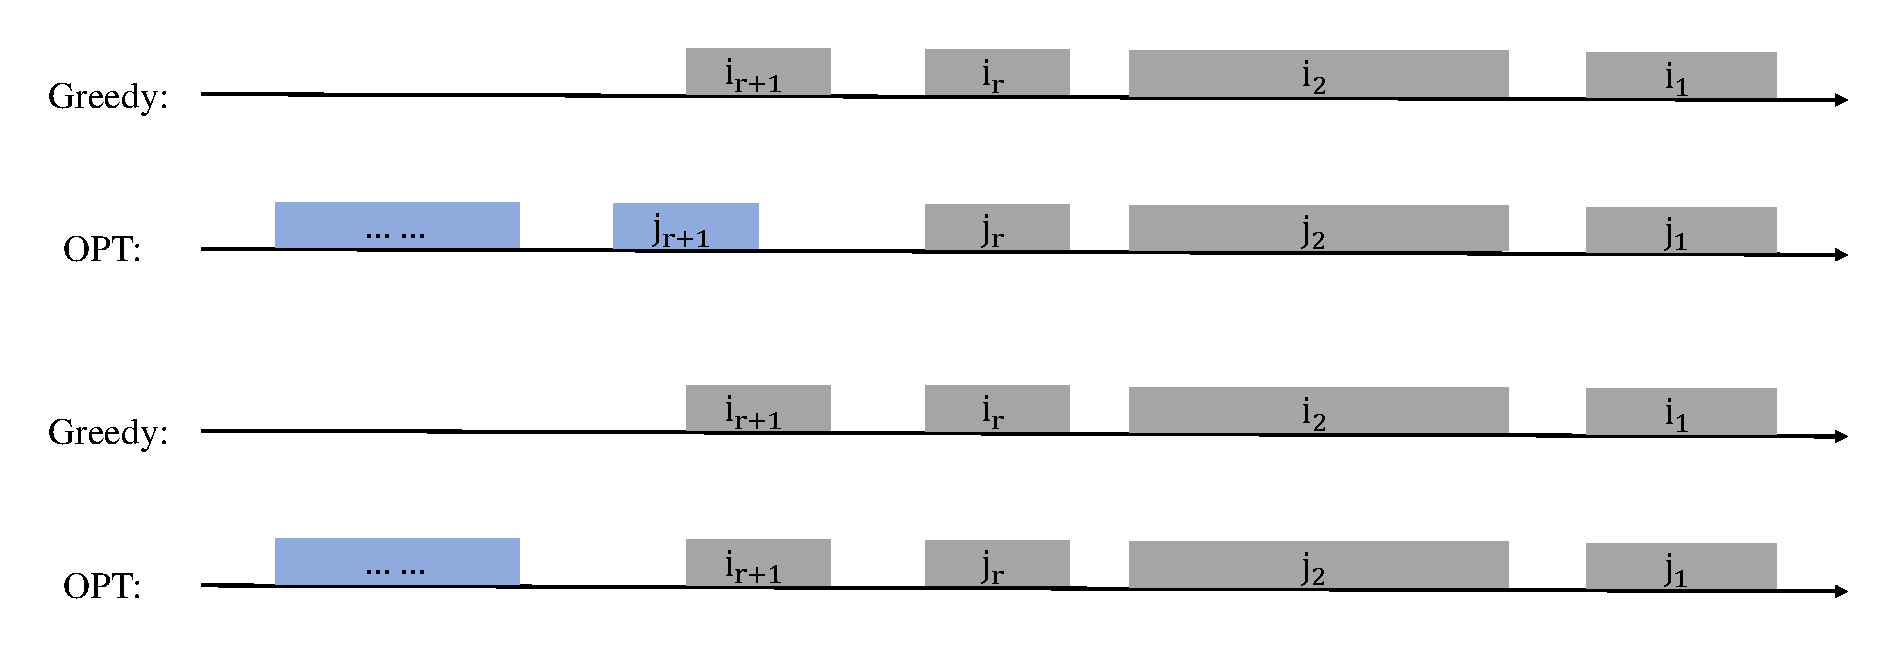
\includegraphics[width=0.7\textwidth]{Fig-Interval_Scheduling.pdf}
                \caption{Correctness Analysis for the Attempt}\label{Fig-Interval-Scheduling}
            \end{figure}
            This attempt is correct, we'll prove this by contradiction.\\
            Assume this greedy strategy is not optimal. Let $i_1,i_2,\dots,i_k$ denote set of jobs selected by greedy. Let $j_1,j_2,\dots,j_m$ denote set of jobs in an optimal solution with $i_1=j_1,i_2=j_2,\dots,i_r=j_r$ for the largest possible value of $r$ ($r<k,r<m$). Since job $i_{r+1}$ starts after $j_{r+1}$, we can replace job $j_{r+1}$ with job $i_{r+1}$ and the solution is still feasible and optimal. That contradicts the maximality of $r$. Thus, this greedy strategy is optimal.
	    \end{solution}
	
	\item \textit{Done deal.} In a basketball league, teams need to complete player trades through matching contracts. Every player is offered a contract. For the sake of simplicity, we assume that the unit is $ M $, and the size of all contracts are integers. The process of contract matching refers to the equation: $ \sum_{i\in A} a_{i}=\sum_{j\in B} b_{j} $, where $ a_{i} $ refers to the contract value of player $ i $ in team $A$ involved in the trade and $ b_{j} $ refers to the value of player $ j $ in team $B$. 
	
	Assume that you are a manager of a basketball team and you want to get \textbf{one} star player from another team through trade. The contract of the star player is $ n (n\in \mathbb{N}^+) $. The goal is to complete the trade with as few players as possible. 
	
	\begin{enumerate}
		\item Describe a \textbf{greedy} algorithm to get the deal done with the least players in your team. Assume that there are only 4 types of contracts in your team: $25M$, $ 10M $, $ 5M $, $ 1M $, and there is no limit to the number of players. Prove that your algorithm yields an optimal solution.
		\item Suppose that the available contract sizes are powers of $c$,
		i.e., the values are $c^{0}, c^{1}, \ldots, c^{k}$ for some integers $c>1$ and $k \geq 1$. Show that the greedy algorithm always yields an optimal solution.
		\item Give a set of contract sizes for which the greedy algorithm does not yield an optimal solution. Your set should include a $ 1M $ so that there is a solution for every value of $ n $.
	\end{enumerate}
    \begin{solution}
        ~
        \begin{enumerate}
            \item \begin{minipage}[t]{0.8\textwidth}
        	    \begin{algorithm}[H]
        		\KwIn{The target $x$}
        		\KwOut{A set of the number of contracts of different sizes}
        		
        		\BlankLine
        		\caption{Greedy Algorithm to Get the Deal Done}\label{greedy-deal}
        		$a_1\leftarrow 0$; $a_2\leftarrow 0$; $a_3\leftarrow 0$; $a_4\leftarrow 0$\;
        	    $c_1\leftarrow 1$; $c_2\leftarrow 5$; $c_3\leftarrow 10$; $c_4\leftarrow 25$\;
        	    $S\leftarrow \varnothing$\;
        		\While{$x\neq 0$ }{
        		let $k$ be largest integer such that $c_k<x$\;
        			\If{$k=0$}{
        				\Return ``no solution found"\;
        			}
        			$x\leftarrow x-c_k$\;
        		    $a_k\leftarrow a_k+1$\;
        		}
        		\Return $S=\{a_1,a_2,a_3,a_4\}$;
        	    \end{algorithm}
                \end{minipage}
                
                ~\\
                The Alg.\ref{greedy-deal} shows the greedy algorithm to get deal done with the least players, which always chooses the player with the largest contract. Then we'll prove that this algorithm will yields an optimal solution.\\
                We denote the number of the players involved in the trade with $c_k$-sized contract by $a_k$. Then we have the properties as below.\\
                \textbf{Property 1.} $a_1<=4$.\\
                \textbf{Proof.}We can replace five $c_1$ with one $c_2$, which involve fewer players.\\
                \textbf{Property 2.} $a_2<=1$.\\
                \textbf{Proof.}We can replace two $c_2$ with one $c_3$, which involve fewer players.\\
                \textbf{Property 3.} $a_3<=2$.\\
                \textbf{Proof.}We can replace three $c_2$ with one $c_1$ and one $c_4$, which involve fewer players.\\
                \textbf{Property 4.} $a_2+a_3<=2$.\\
                \textbf{Proof.}We can replace one $c_2$ and two $c_3$ with one $c_4$, which involve fewer players.\\
                ~\\
                We continue the proof by induction on $x$. Consider an optimal way to change $c_k<k<c_{k+1}$ and greedy takes a $c_k$-sized contract. We claim that any optimal solution must also take $c_k$-sized contract. If not, it needs enough contracts of type $c_1,\dots,c_{k-1}$ to add up to $x$. However, due to the properties above, we have
                \begin{align}
                    \begin{split}
                        \sum_{i=1}^{i=1}a_ic_i = 4<c_2\\
                        \sum_{i=1}^{i=2}a_ic_i = 9<c_3\\
                        \sum_{i=1}^{i=3}a_ic_i = 24<c_4\\
                    \end{split}
                \end{align}
                Thus, any optimal solution must also take a $c_k$-sized contract. Problem reduces to get a $(x-c_k)$-sized deal done, which, by induction, is optimally solved by greedy algorithm.
                
                \item Similar to problem a, we define the original problem as $P(x)$. 
                For an optimal solution $S=\{a_0,...,a_k\}$, we have $x = a_0\times c_0+...+a_k\times c_k$ where $ c_i = c^{i}$. 
                According to problem a, we have $a_0,...,a_{k-1}<=c-1$. 
                So, $a_0\times c_0+...+a_{k-1}\times c_{k-1}<=(c-1)\times \frac{1-c^{k}}{1-c}=c^{k}-1<c^{k}$.
                That ensures if $x\ge c_k$, any optimal solution must take a $c_k$-sized contract.
                So the original problem is reduced to find the solution to $P(x-c_k)$, which, by induction, is optimally solved by greedy algorithm.
                Therefore, the greedy algorithm always yields an optimal solution.
                
                \item Let the set of contract sizes $D = \{10M,7M,1M\}$. 
                When we use greedy algorithm to get a $14M$-sized deal done.
                The answer will be one $10M$-sized contract and four $1M$-sized contracts, which involves 5 players.
                However, the globally optimal solution is two $7M$-sized contracts, which involves only 2 players.
        \end{enumerate}
    \end{solution}
    
	
    \item \textit{Set Cover.} \textbf{Set Cover} is a typical kind of problems that can be solved by greedy strategy. One version is that: Given $n$ points on a straight line, denoted as $\{x_i\}_{i=1}^n$, and we intend to use minimum number of closed intervals with fixed length $k$ to cover these $n$ points.
    \begin{enumerate}
    	\item Please design an algorithm based on \textbf{greedy} strategy to solve the above problem, in the form of \emph{pseudo code}. Then please analyze its \emph{worst-case} complexity.
    	\item Please prove the correctness of your algorithm.
    	\item Please complete the provided source code by C/C++ {\color{blue}(The source code \emph{Code-SetCover.cpp} is attached on the course webpage)}, and please write down the output result by testing the following inputs: 
    	\begin{enumerate}
    		\item the number of points $n=7$;
    		\item the coordinates of points
    		$x=\{1,2,3,4,5,6,-2\}$;
    		\item the length of intervals
    		$k=3$.
    	\end{enumerate}
        \textbf{Remark}: Screenshots of running results are also acceptable 
    \end{enumerate}
    \begin{solution}
        ~\\
        \begin{enumerate}
        \item 
        
        \begin{minipage}[t]{0.8\textwidth}
        	    \begin{algorithm}[H]
        		\KwIn{The $n$ points on a straight line $\{x_i\}_{i=1}^n$ and the length of intervals $k$}
        		\KwOut{The minimum number of closed intervals to cover these $n$ points}
        		
        		\BlankLine
        		\caption{Greedy Algorithm to Solve the Set Cover Problem}\label{greedy-deal}
        		Sort the $n$ points so that $x_1\leq x_2 \leq \dots \leq x_n$\;
        	    $r\leftarrow -\infty$\;
        	    $i\leftarrow 1$\;
        	    $count \leftarrow 0$\;
        		\While{$i\leq n$ }{
        			\If{$r<x_i$}{
        				$r \leftarrow x_i + k$\;
        				$count \leftarrow count+1$\;
        			}
        			$i \leftarrow i+1$\;
        		}
        		\Return $count$;
        	    \end{algorithm}
                \end{minipage}
                ~\\
            In the strategy shown above, we choose the smallest point as the starting point of the first interval. And at every time, we choose the smallest point which has not been covered to be the starting point.\\
            \textbf{Worst-case complexity:} If we use $QuickSort$, then the worst-case time complexity is $O(n^2)$. However, if we use sorting algorithm like $MergeSort$, the worst-case time complexity will be $O(n\log n)$. The while loop has a time complexity of $O(n)$. Thus, the worst-case time complexity is $O(n\log n)$ or $O(n^2)$ depending on the sorting algorithm we choose. Also, the sorting algorithm determine the worst-case space complexity. If we choose a local sorting algorithm, when the worst-case space complexity will be $O(1)$.
        \item 
        ~
        \begin{figure}[htbp]
                \centering
                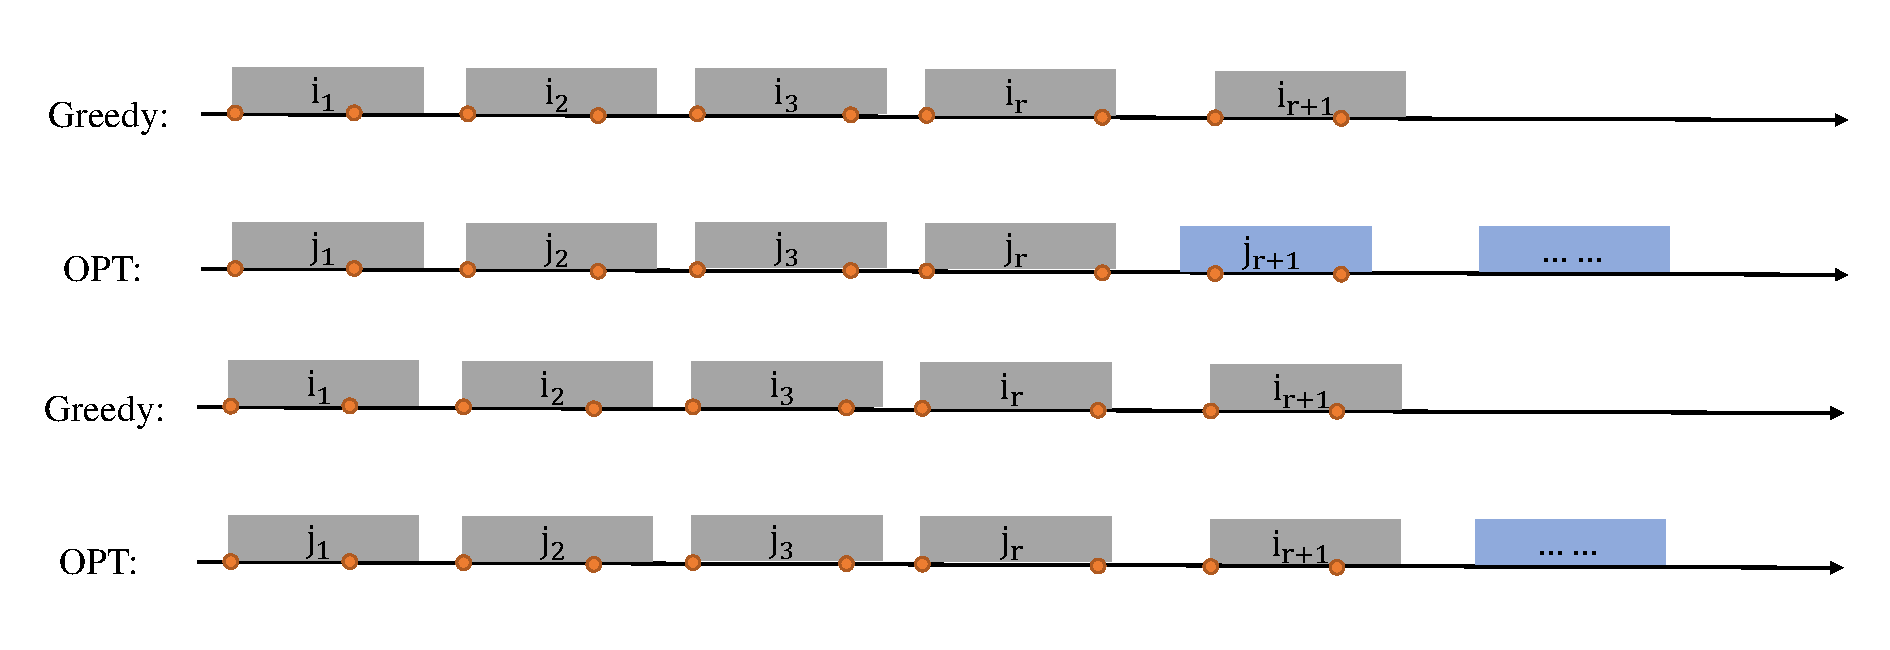
\includegraphics[width=0.7\textwidth]{Fig-Set_Cover.pdf}
                \caption{Correctness Analysis for the Greedy Algorithm to Solve the Set Cover Problem}\label{Fig-Interval-Scheduling}
            \end{figure}
        Similar to problem 1, we can prove by contradiction. Assume that this greedy strategy is not optimal. Let $i_1,i_2,\dots,i_k$ denote the set of intervals selected by greedy. Let $j_1,j_2,\dots,j_m$ denote set of intervals in an optimal solution with $i_1=j_1,i_2=j_2,\dots,i_r=j_r$ for the largest possible value of $r$ ($r<k,r<m$). Since the starting point of $i_{r+1}$ is the smallest point which is not covered by $i_1,i_2,\dots,i_r$, we can replace interval $j_{r+1}$ with interval $i_{r+1}$ and the solution is still feasible and optimal. That contradicts the maximality of $r$. Thus, the greedy strategy is optimal.
        \item 
        Please refer to \emph{Code-SetCover.cpp}.
        The running results are listed as below.
        \begin{figure}[htbp]
                \centering
                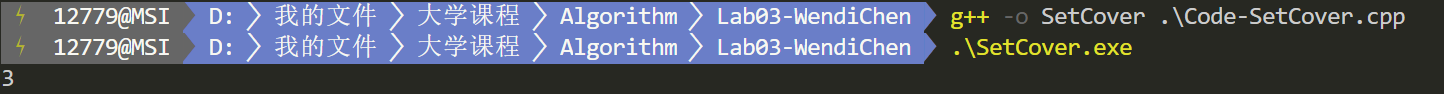
\includegraphics[width=0.7\textwidth]{Fig-SetCover_Result.png}
                \caption{Running Result of the Greedy Algorithm to Solve the Set Cover Problem}\label{Fig-Interval-Scheduling}
            \end{figure}
        \end{enumerate}
    \end{solution}
    
\end{enumerate}



\vspace{20pt}

\textbf{Remark:} You need to include your .pdf and .tex files in your uploaded .rar or .zip file.

%========================================================================
\end{document}
